\chapter{Phytoscheme} \label{phytoscheme}
\section{Contexto y necesidades reales} \label{phytoscheme.contexto}
Los productos fitosanitarios son un elemento imprescindible en la producción agrícola, tanto en los sistemas convencionales de agricultura como en los sistemas de agricultura integrada o ecológica. Sin su existencia, muchos cultivos de las zonas de producción de mayor interés económico y social serían inviables hoy en día debido a los estragos potenciales de las diferentes clases de plagas.\par
No obstante, el uso de dichos productos fitosanitarios debe estar regulado ya que una aplicación indebida de los mismos puede tener otros efectos no deseables. Dichos efectos de ninguna manera deben suponer un peligro para la salud humana y tampoco riesgos inaceptables para el medio ambiente. \par
Por ello el Estado sólo aprueba la comercialización de aquellos productos fitosanitarios que sean útiles para combatir las plagas pero no impliquen otros riesgos colaterales. Para que un \gls{fito} pueda comercializarse debe estar inscrito necesariamente en el Registro Oficial de Productos Fitosanitarios - \textit{Página web del ministerio de agricultura y pesca, alimentación y medio ambiente de España} \cite{mapama}\par
Es, por tanto, necesario y casi obligatorio que la información del Registro de Productos Fitosanitarios llegue de manera precisa a todos los implicados en el área del uso de los productos fitosanitarios\par
La \textit{Directiva 2009/128/CE} \cite{directiva128} establece el marco de la actuación comunitaria para conseguir un uso sostenible de los productos fitosanitarios. Esta Directiva implica, por ejemplo, la obligación del registro del uso de productos fitosanitarios. Un ejemplo del desarrollo de esta Directiva es el \textit{Cuaderno de Explotación} \cite{cuadernoexplotacion}. Este cuaderno aglutina de manera ordenada y armonizada todos los elementos que deberán registrar los titulares de las explotaciones agrícolas, con el objetivo de facilitar el cumplimiento de la Directiva.\par
Actualmente, hay varias empresas que ofrecen aplicaciones (p. ej. \textit{aGROSLab} \cite{agroslab}, \textit{Agricolum} \cite{agricolum} o el \textit{Cuaderno de Campo Agronev} \cite{agronev}) que implementan el Cuaderno de Explotación. Un valor añadido que suelen incorporar estas aplicaciones es una base de datos con información acerca de los productos fitosanitarios autorizados. El problema al que se enfrentan estas empresas es que esta información no se publica de forma uniforme en toda la Unión Europea. Es decir, hay al menos un publicador por país miembro, la información publicada es heterogénea y los formatos normalmente son difícilmente accesibles. Además, a nivel Europeo, hay una \textit{base de datos de referencia} \cite{pesticidesdb} de las restricciones más o menos comunes en el uso de productos fitosanitarios. Dado que no hay un estándar de publicación establecido, una consecuencia adicional de esta situación es que es complicado verificar si un producto tratado con una serie de productos fitosanitarios en un país miembro puede ser exportado a otro, ya que la normativa fitosanitaria aplicable puede diferir.\par
En cuanto a la importación de productos desde un país miembro de la Unión Europea, el artículo 52 del \textit{Reglamento (CE) 11/07/2009} \cite{reglamento} se refiere a este trámite como comercio paralelo y se especifica que para poder llevarlo a cabo, el Estado Miembro donde se desee introducir deberá determinar que el producto fitosanitario es idéntico en composición a otro ya autorizado en su territorio al que se denominará “producto de referencia”. Para realizar el trámite, actualmente el proceso consta en rellenar la \textit{solicitud} del \gls{certificado} \cite{solicitud} (disponible en la página web del ministerio), entregarla a la Subdirección General de Higiene Vegetal y Forestal y esperar a que sea aprobada - \textit{Preguntas frecuentes Mapama} \cite{faqmapama} \par
Los principales problemas actuales de este proceso vienen por una parte en el lado del agricultor/empresa que solicita la importación puesto que no solo el tiempo de respuesta en ocasiones puede ser muy largo (de hasta de 45 días - Artículo 52, punto 2 del Reglamento (CE) 11/07/2009) sino que además, el agricultor o bien tiene poca información acerca de los productos permitidos en una importación/exportación o el acceso a dicha información es bastante tedioso y complicado. Por otra parte en el lado de la institución certificadora encargada de comprobar la solicitud el proceso no es del todo eficiente debido al hecho de tener que verificar manualmente si el producto cumple con los requisitos de composición del correspondiente producto en el país de importación/exportación. Estos problemas se pueden observar claramente en el siguiente diagrama, que muestra un flujo típico en un trámite de comercio paralelo entre un agricultor/empresa que quiere importar un producto a un determinado país, en este caso, España: 

\begin{figure}[H]
    \centering
    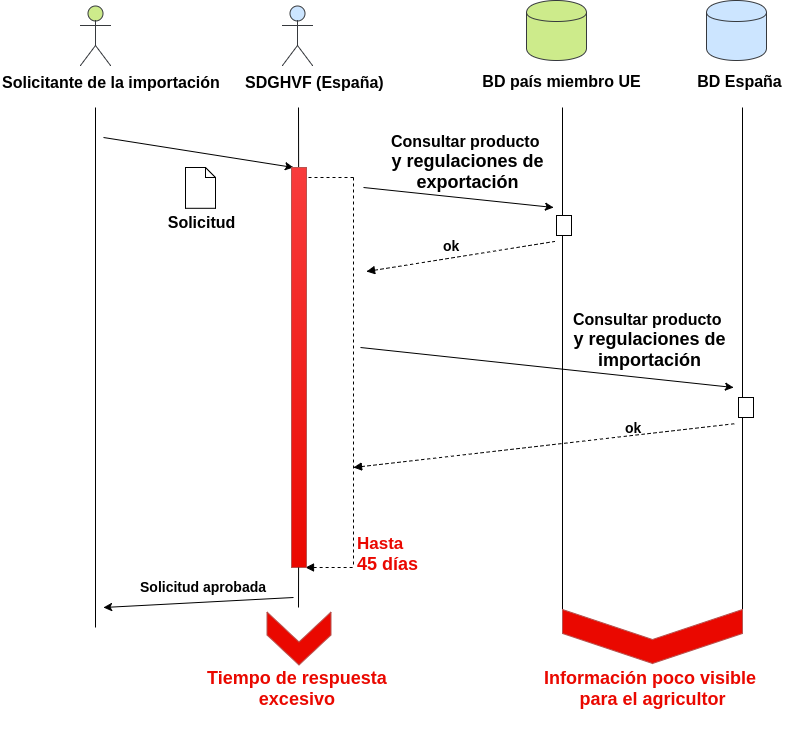
\includegraphics[width=1\textwidth,height=14cm]{Imagenes/Diagrama_de_flujo_proceso_actual_de_importacion_producto_fitosanitario}
    \caption{Diagrama de flujo del proceso actual de importación de un producto fitosanitario}
    \label{fig:flujo_actual_importacion}
\end{figure}
\par
*SGHVF = Subdirección General de Higiene Vegetal y Forestal\\\par
Es razonable desarrollar un sistema que provea un esquema único donde los datos estuvieran integrados y congruentes entre los diferentes países de la unión europea para facilitar un consumo posterior por las aplicaciones, e, incluso, directamente por los agricultores. 

\section{Motivación y objetivos} \label{phytoscheme.motivacion}
Habiendo visto el panorama descubierto en el apartado anterior, era evidente que se podían introducir mejoras al proceso actual que pueden beneficiar a las partes involucradas (tanto a agricultores y empresas como a las instituciones reguladoras). Con ese objetivo en mente, se propone desarrollar una aplicación prototipo que valide el proceso de integración de la información de diferentes países en un esquema único que recogiese los datos que de otra manera tendrían que ser recopilados manualmente, con largos tiempos de espera y con una incertidumbre por parte de los agricultores/empresas en lo que a datos sobre productos fitosanitarios respecta.\par 
El siguiente diagrama muestra el potencial proceso que tendría que seguir una persona interesada en realizar una importación y los problemas que sería capaz de solucionar el desarrollo de la aplicación planteada en este proyecto:

\begin{figure}[H]
    \centering
    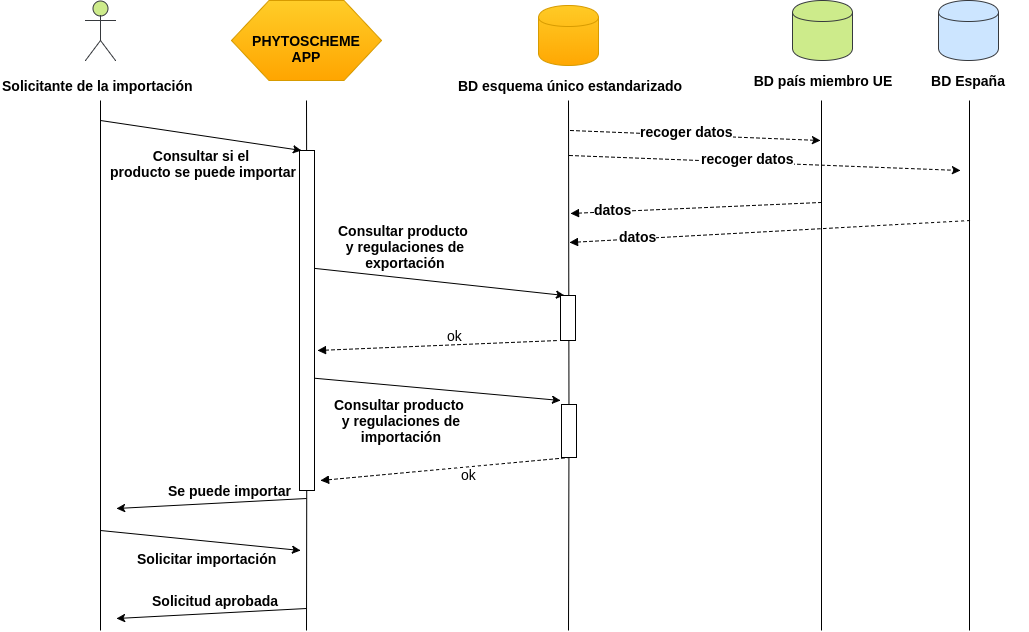
\includegraphics[width=1\textwidth,height=11cm]{Imagenes/Diagrama_de_flujo_proceso_potencial_de_importacion_producto_fitosanitario}
    \caption{Diagrama de flujo del potencial  proceso de importación de un producto fitosanitario}
    \label{fig:flujo_potencial_importacion}
\end{figure}
\par

Se puede apreciar que con este desarrollo se conseguiría no solo reducir los plazos de respuesta al agricultor/empresa sino también una mayor transparencia en la consulta de los datos, puesto que al estar integrados en un modelo único, el agricultor/empresa o los interesados podrían tener acceso a toda la información y consultar cualquier aspecto que de otra manera habría sido prácticamente inaccesible. No solo eso, sino que además, al conseguir un modelo potencialmente estandarizado, no haría falta del trabajo manual y tedioso de comprobación de los requisitos por parte de la Subdirección General de Higiene Forestal y Vegetal sino que sería el propio sistema el encargado de comprobar si la petición del solicitante cumple con la \textit{\gls{legisfito}} vigentede cada país. \par
Uno de los aspectos a tener en cuenta al comienzo del proyecto fue el hecho de que para que la solución se pudiera aplicar a un nivel real del problema, se necesitaba una gran capacidad de almacenamiento. Los datos deberían almacenarse periódicamente y además, potencialmente podrían provenir de multitud de fuentes, en diferentes formatos, con unos tamaños variables y constantes actualizaciones. Muchas fuentes equivalen a muchos datos, y muchos datos equivalen a la necesidad de un sistema de almacenamiento capaz de soportar toda esa carga. 
\par
Unido a esto, la elección de dicho sistema de almacenamiento suponía un punto crítico, puesto que no bastaría con cualquier base de datos sino que tendría que cumplir ciertas características como la posibilidad de guardar los datos en sus formatos originales, la necesidad de generar una jerarquía para su almacenamiento, o la posibilidad de integración con los trabajos de transformación y procesado de los datos. 
\par
Por ello, el proyecto tuvo como objetivo principal desarrollar una solución prototipo para demostrar la validez de los procesos y herramientas involucradas en la integración de varias fuentes heterogéneas de productos fitosanitarios en un modelo único.

\section{Restricciones} \label{phytoscheme.restricciones}
\par
Teniendo en cuenta que el proyecto actual es un TFG y no un proyecto comercial, se tienen que tomar en cálculo una serie de restricciones que vienen dadas tanto por la naturaleza del proyecto como por los partícipes del mismo. En primer lugar, siendo un TFG, debe realizarse una cantidad de esfuerzo equivalente a 12 ECTS.. Dado que el desarrollo realizado en este proyecto está enfocado a formar parte de un plan mucho mayor, donde el trabajo realizado se retomará y ampliará en futuros TFG, desde el principio se delimitaron aquellas características que se deseaban incluir en el proyecto y también aquellas que no corresponden a esta iteración.  Siendo una fase temprana de dicho plan maestro, a esta fase le correspondía la parte de validación del modelo, de las tecnologías empleadas y de la viabilidad del producto, no siendo primordial tener un producto final robusto sino demostrar que las tecnologías en su totalidad se complementaban y funcionaban acorde a lo esperado. 
\par
Otro factor restrictivo dada la naturaleza del proyecto es el hecho de que existe un director, que puede marcar las pautas de desarrollo, sugerir e imponer metodologías de trabajo o incluso herramientas del stack tecnológico que pueden suponer una ventaja o una desventaja en el desarrollo del proyecto. El alumno debe ser capaz de discutir estas tendencias con el director y razonar las decisiones que se tomen, en conjunto, y exponiendo sus puntos de vista con el objetivo de llegar a un acuerdo común. 

\section{Requisitos - Técnica \textit{\gls{moscow}}} \label{phytoscheme.requisitos}
\par 
Por imposición y recomendación del director del proyecto, el análisis y la captura de requisitos han estado desde el principio  regidos por el método \textit{\gls{moscow}}, una técnica de priorización de requisitos usada en la gestión de proyectos, análisis de negocio y desarrollo de software con objetivo de llegar a un acuerdo común con los \textit{stakeholders} (integrantes del proyecto) sobre la importancia que se debería dar a cada requisito. Esta técnica también es conocida bajo los nombres de \textit{priorización \gls{moscow}} o \textit{análisis \gls{moscow}}.
\par
La metodología \textit{\gls{moscow}} dicta cuatro categorías mediante las que se pueden priorizar los requisitos de un sistema o proyecto: 

\begin{enumerate}
\item \textbf{Debe tener:} Son aquellos requisitos críticos para que el trabajo realizado durante un periodo de tiempo determinado (en nuestro caso desde ahora hasta junio 2017) sea considerado un éxito (\textit{TFG} aprobado). Si uno de estos requisitos no se incluye, el proyecto debera ser considerado un fallo (no se puede presentar el \textit{TFG}). \textit{Debe tener} en \textit{\gls{moscow}} se refiere a \textit{MUST}, que puede ser considerado un acrónimo de \textit{Minimum Usable SubseT}. En ese sentido se puede entender como la unión de los requisitos del producto mínimo viable con los requisitos legales (p.ej. documentación en forma de memoria de \textit{TFG}, cumplimiento \textit{LOPD}, etc.) y de seguridad (en el sentido de robustez y calidad de la solución) obligatorios o acordados. Los requisitos del proyecto acordados para esta categoría han sido los siguientes: 
\begin{itemize}
\item Recolectar datos oficiales tanto de productos fitosanitarios autorizados de España como de las sustancias activas a nivel europeo. 
\item Almacenar la última versión de los datos en formato original y además mantener todas las versiones descargadas. 
\item Monitorizar y almacenar los procesos de recolección de los datos de entrada así como las rutas de su procesado.
\item Ofrecer la infraestructura y las herramientas de configuración necesarias para una expansión futura del proyecto. 
\item Implementar un modelo de aplicación consistente, ejemplificando el ciclo de vida típico de los datos desde su recogida hasta su presentación visual. 
\item Una memoria extensa y detallada. 
\end{itemize}

\item \textbf{Debería tener:} Son aquellos que son importantes pero no necesarios para ser realizados durante el periodo de tiempo determinado. Pueden posponerse para ser realizados en el siguiente periodo. Son vitales pero no obligatorios, si no se implementan la solución es viable pero es doloroso no hacerlo. En el caso de nuestro proyecto, dentro de esta categoría se han identificado los siguientes requisitos: 
\begin{itemize}
\item Mecanismo de control de esfuerzos.
\item Mecanismo de control de versiones.
\item Módulo de trazabilidad de los datos desde las fuentes originales hasta su visualización. 
\item Mecanismo de detección de errores e inconsistencias en los datos provenientes de diferentes fuentes. 
\end{itemize}


\item \textbf{Podría tener:} Son aquellos que comparados con los anteriores son los menos deseados o tienen menor impacto. Hay que tenerlos controlados ya que sólo se podrán entregar si se dan las mejores condiciones (por ejemplo, el proyecto va más rápido de los esperado). Si hay algún riesgo en la entrega del proyecto estos requisitos serían los primeros en ser descartados. A continuación se pueden ver los requisitos del proyecto que se han ubicados dentro de esta categoría:

\begin{itemize}
\item Genericidad en cuanto al soporte de integración de los datos de diferentes fuentes basado en un fichero de claves y valores. 
\item Soporte para la búsqueda de registros (datos) desde la interfaz web. 
\item Desarrollo dirigido por un paradigma de inversión de independencias para conseguir un control centralizado.
\end{itemize}

\item \textbf{No tendrá:} Son aquellos que no van a ser entregados durante el periodo considerado. Se mantienen en esta lista de alcance para clarificar el alcance de la solución. Esto evita que informalmente sean introducidos más tarde. El objetivo de esta categoría es ayudar a mantener el foco en una solución estricta. 


\begin{itemize}
\item Rediseño y desarrollo en el lado del \textit{Front-End}.
\item Desarrollo de tests adicionales en el proyecto de \textit{JHipster}
\item Integración de más de dos fuentes de datos heterogéneas. 
\end{itemize}


\end{enumerate}



